\chapter{ИССЛЕДОВАТЕЛЬСКАЯ ЧАСТЬ}

В данном разделе будут представлены характеристики компьютера, на котором проводилось исследование. Также в данном разделе будут приведено описание и постановка исследования. Будут приведены результаты сравнения времени вставки игры в таблицу в зависимости от количества игр и от того, где происходит преобразование строки, содержащей информацию о жанрах, в xml-формат на уровне приложения или на уровне базы данных.

\section{Технические характеристики устройства}

Технические характеристики устройства, на котором выполнялись измерения:

\begin{itemize}
	\item[---] процессор --- AMD Ryzen 5 4600H с Radeon Graphics 3.00 ГГц~\cite{proc};
	\item[---] операционная система --- Windows 10 Корпоративная 22H2;
	\item[---] оперативная память --- 24 Гб;
	\item[---] количество логических ядер --- 12;
	\item[---] ёмкость диска --- 512 GB;
\end{itemize}

Во время тестирования ноутбук был включен в сеть питания и нагружен только приложениями встроенными в операционную систему и системой тестирования. Сторонние приложения запущены не были.

\section{Описание исследования}

Цель эксперимента - исследовать зависимость по времени добавления игр в таблицу от их количества и от реализации алгоритма преобразования строки, содержащей информацию о жанрах, в xml формат --- на уровне приложения или на уровне базы данных. 

В ходе исследования анализируется время, затрачиваемое на вставку игр в таблицу в зависимости от их количества и от реализации алгоритма преобразования строки, содержащей информацию о жанрах, в xml формат. Для каждого количества игр было проведено 50 измерений и вычислено среднее арифметическое.

В исследовании для каждой реализации алгоритма преобразования строки в xml формат измеряется время вставки различного количества игр в таблицу. Каждой игре добавляется 20 жанров.

\section{Результаты исследования}

В таблице~\ref{tbl:experiment1} приведены результаты исследования. 

\begin{table}[H]
	\centering
	\captionsetup{justification=raggedleft, singlelinecheck=false}
	\caption{Результаты исследования зависимости времени (мс), затрачиваемого на вставку в игр таблицу, от количества и реализации алгоритма}
	\label{tbl:experiment1}
	\begin{tabular}{|l|l|l|} 
		\hline
		\multirow{2}{*}{Количество игр} & \multicolumn{2}{l|}{Реализация алгоритма}\\\cline{2-3}
		&на стороне базы данных& на стороне приложения\\\hline
		100	&~1116,7&	~~678,8\\\hline
		200	&~1347,0&	~1358,1\\\hline
		300	&~2045,2&	~2585,2\\\hline
		400	&~4576,3&	~4851,6\\\hline
		500	&~9162,1&	~8373,2\\\hline
		600	&10861,2&	13313,7\\\hline
		700	&14750,6&	18671,4\\\hline
		800	&15918,4&	21309,9\\\hline
		900	&23513,6&	31194,5\\\hline
		1000	&39439,7&	45007,0\\\hline
		
	\end{tabular}
\end{table}

На рисунке~\ref{img:experiment1} представлены графики зависимости времени вставки игр в таблицу от реализации алгоритма и от количества добавляемых игр.

\begin{figure}[H]
	\centering

	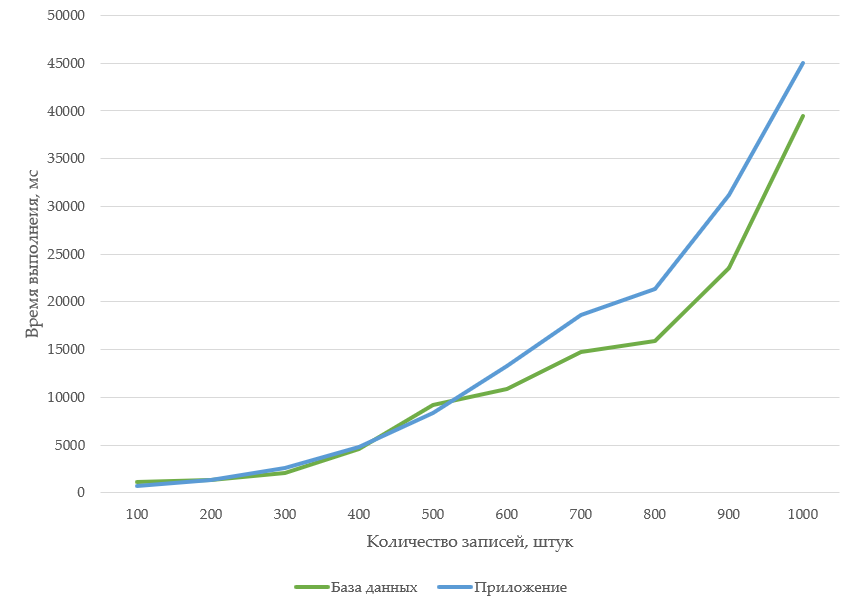
\includegraphics[scale=0.8]{../imgs/experiment.png}
	\captionsetup{justification=centering}
	\caption{Зависимость времени вставки игр в таблицу от реализации алгоритма и от количества добавляемых игр}
	\label{img:experiment1}
\end{figure}

Результаты показывают, что добавление игр в таблицу с помощью алгоритма преобразования строки в xml формат, реализованного на уровне базы данных, более эффективно, чем добавление игр с помощью алгоритма, реализованного на уровне приложения. Для добавления 800 игр реализация на уровне базы данных примерно на 25\% быстрее, чем реализация на уровне приложения.

При реализации вставки на стороне базы данных в процедуру передается одна запись, и СУБД выполняет все вычисления, в то время как приложение должно сначала получить таблицу, в которую должна быть выполнена вставка, затем преобразовать строки в формат xml и, наконец, вставить преобразованную запись в таблицу.  

\section{Вывод}

Результаты показывают, что при фиксированном количестве игр для вставки игр в таблицу требуется больше времени, когда алгоритм выполняется на уровне приложения, чем когда он выполняется на уровне базы данных. Таким образом, видно, что на время выполнения влияет не то, выполняется ли алгоритм на уровне базы данных или на уровне приложения, а объем данных, которые передаются из базы данных в приложение и обратно.


